% Copyright 2004 by Till Tantau <tantau@users.sourceforge.net>.
%
% In principle, this file can be redistributed and/or modified under
% the terms of the GNU Public License, version 2.
%
% However, this file is supposed to be a template to be modified
% for your own needs. For this reason, if you use this file as a
% template and not specifically distribute it as part of a another
% package/program, I grant the extra permission to freely copy and
% modify this file as you see fit and even to delete this copyright
% notice. 

\documentclass{beamer}

\usepackage{bibentry}

\usepackage{graphicx}
\usepackage[portuguese]{babel} % Para termos legendas em português


% There are many different themes available for Beamer. A comprehensive
% list with examples is given here:
% http://deic.uab.es/~iblanes/beamer_gallery/index_by_theme.html
% You can uncomment the themes below if you would like to use a different
% one:
%\usetheme{AnnArbor}
%\usetheme{Antibes}
%\usetheme{Bergen}
%\usetheme{Berkeley}
%\usetheme{Berlin}
%\usetheme{Boadilla}
%\usetheme{boxes}
%\usetheme{CambridgeUS}
%\usetheme{Copenhagen}
%\usetheme{Darmstadt}
%\usetheme{default}
%\usetheme{Frankfurt}
%\usetheme{Goettingen}
%\usetheme{Hannover}
%\usetheme{Ilmenau}
%\usetheme{JuanLesPins}
%\usetheme{Luebeck}
\usetheme{Madrid}
%\usetheme{Malmoe}
%\usetheme{Marburg}
%\usetheme{Montpellier}
%\usetheme{PaloAlto}
%\usetheme{Pittsburgh}
%\usetheme{Rochester}
%\usetheme{Singapore}
%\usetheme{Szeged}
%\usetheme{Warsaw}

\title{A survey into CDNs Security}


\author{Costa, Lucas B.\inst{1} \and Maziero, Carlos A.\inst{2}}

\institute[Universidade Federal do Paran\'a] % (optional, but mostly needed)
{
  \inst{1}%
  Departamento de Inform\'atica\\
  UFPR
}
\date{Dezembro, 2018}


% If you have a file called "university-logo-filename.xxx", where xxx
% is a graphic format that can be processed by latex or pdflatex,
% resp., then you can add a logo as follows:

% \pgfdeclareimage[height=0.5cm]{university-logo}{university-logo-filename}
% \logo{\pgfuseimage{university-logo}}

% Delete this, if you do not want the table of contents to pop up at
% the beginning of each subsection:
\AtBeginSubsection[]
{
  \begin{frame}<beamer>{Sum\'ario}
    \tableofcontents[currentsection,currentsubsection]
  \end{frame}
}

% Let's get started
\begin{document}

\begin{frame}
  \titlepage
\end{frame}

\begin{frame}{Sum\'ario}
  \tableofcontents
  % You might wish to add the option [pausesections]
\end{frame}

% Section and subsections will appear in the presentation overview
% and table of contents.
\section{Introdu\c{c}\~ao}

\subsection{Contextualiza\c{c}\~ao}

\begin{frame}{Contextualiza\c{c}\~ao}
\begin{figure} 
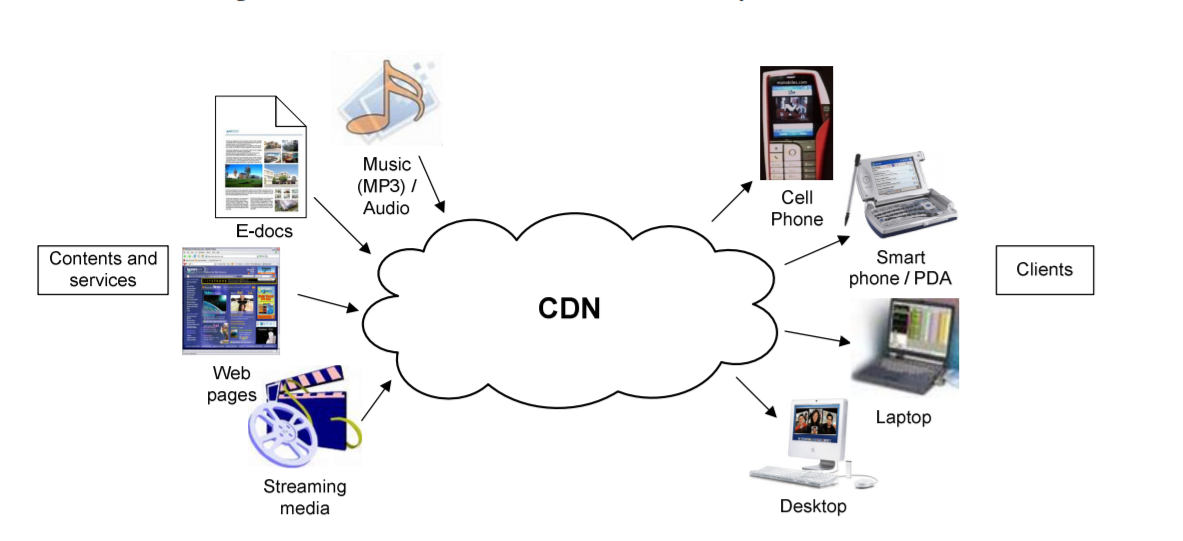
\includegraphics[width=13cm]{Figuras/contextualizacao.png} % leia abaixo
\label{figura:contextualizacao} 
\end{figure}
\end{frame}

\subsection{Composi\c{c}\~ao de uma CDN}

% You can reveal the parts of a slide one at a time
% with the \pause command:
\begin{frame}{Composi\c{c}\~ao de uma CDN}
  \begin{itemize}
  \item {
    Organiza\c{c}\~ao.
    \pause
  }
  \item {   
    Tipos de servidores.
  }
  % You can also specify when the content should appear
  % by using <n->:
  \item<3-> {
    Tipos de relacionamentos.
  }
  \item<4-> {
    Protocolos de intera\c{c}\~oes.
  }
  % or you can use the \uncover command to reveal general
  % content (not just \items):
  \item<5-> {
    Tipos de conte\'udos.
  }
  \end{itemize}
\end{frame}

\section{Composi\c{c}\~ao de uma CDN}

\subsection{Tipos de servidores}
\begin{frame}{Tipos de servidores}
\begin{itemize}
	\item Servidor de origem
	\item Servidor de ponta
\end{itemize}
\begin{figure} 
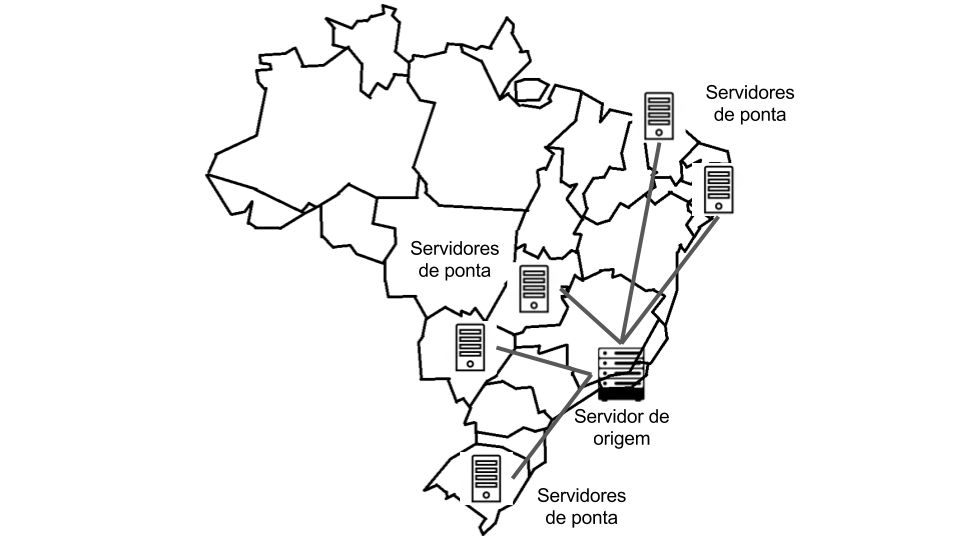
\includegraphics[width=10cm]{Figuras/tipos_servidores.png} 
\label{figura:tipos_servidores} 
\end{figure}
\end{frame}


\subsection{Protocolos de intera\c{c}\~oes}

\begin{frame}{Protocolos de intera\c{c}\~oes} 
\begin{figure} 
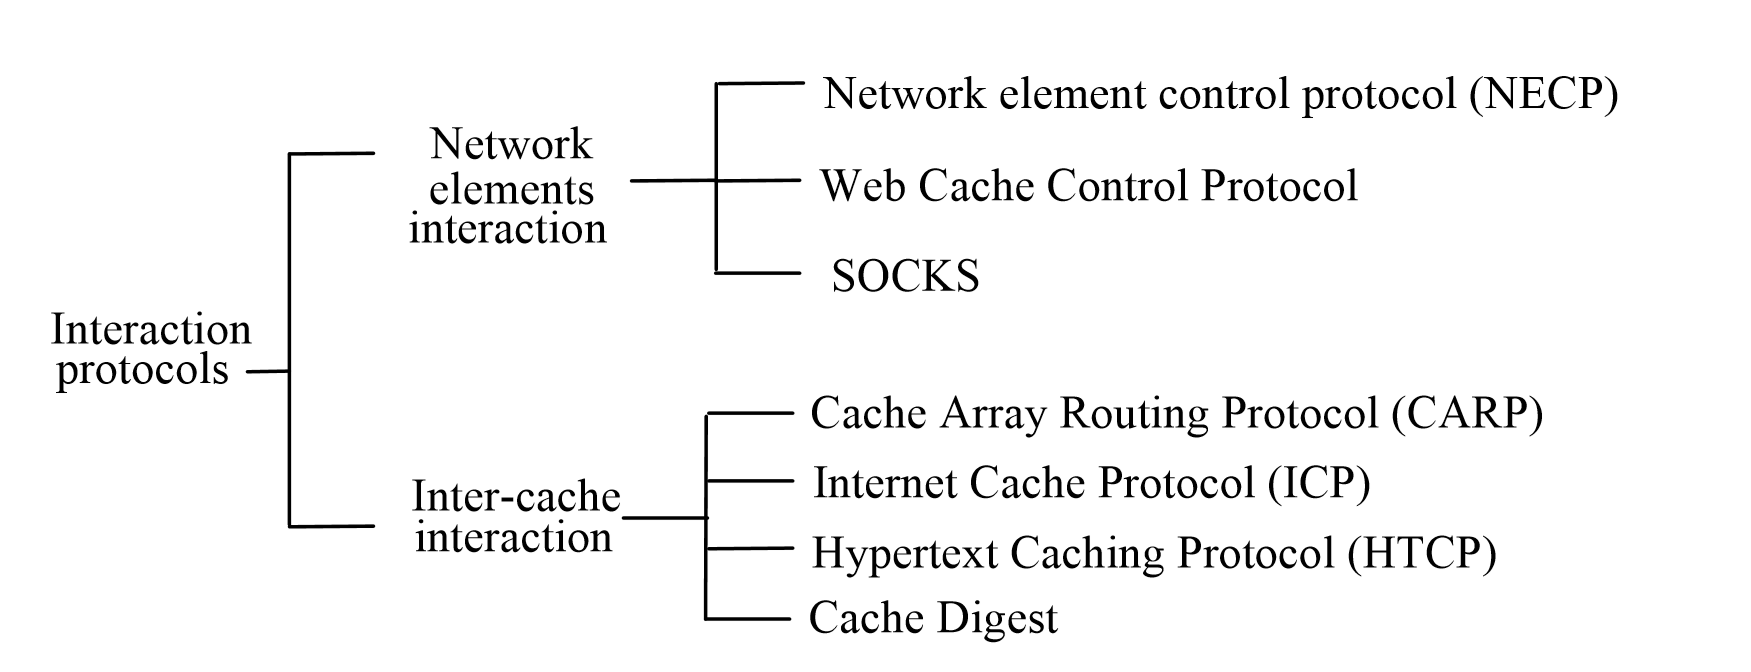
\includegraphics[width=13cm]{Figuras/tipos_relacionamentos.png} 
\label{figura:tipos_relacionamentos}
\end{figure}
\end{frame}

\begin{frame}{Protocolos de intera\c{c}\~oes}{Intera\c{c}\~oes dos elementos da rede}
\begin{figure} 
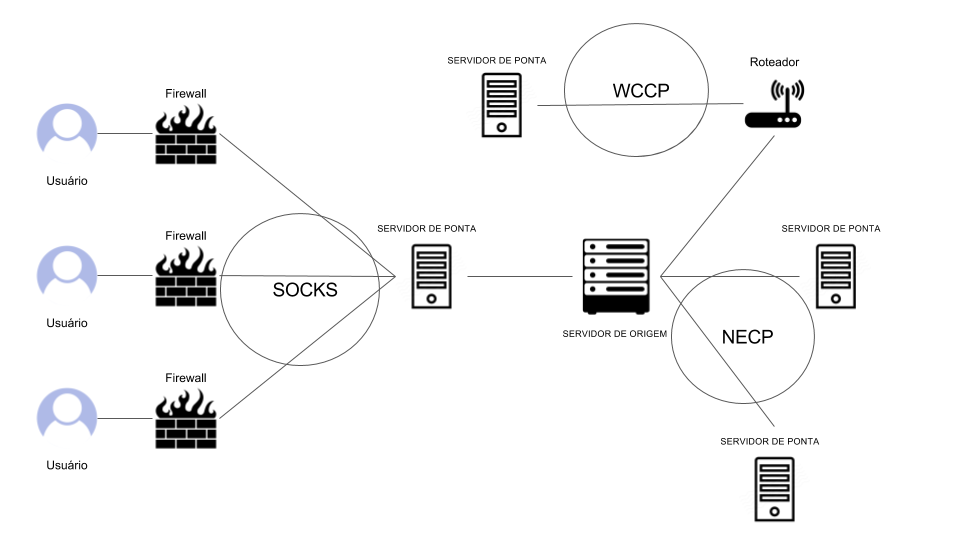
\includegraphics[width=13cm]{Figuras/protocolos_interacao_elementos.png} 
\label{figura:protocolos_interacao_elementos}
\end{figure}
\end{frame}

\begin{frame}{Protocolos de intera\c{c}\~oes}{Intera\c{c}\~oes de cache}
HTCP - Hypertext Caching Protocol
\begin{itemize}
\item Protocolo para descobri Caches HTTP;
\item Suporte ao HTTP 1.0;
\item Permite incluir cabeçalhos nas respostas;
\item Podem ser enviados via TCP/UDP;
\item Devem ser resilientes \`a falhas.
\end{itemize}
\end{frame}

\begin{frame}{Protocolos de intera\c{c}\~oes}{Intera\c{c}\~oes de cache}
ICP - Internet Cache Protocol
\begin{itemize}
\item Protocolo de mensagem leve;
\item Utilizado para comunica\c{c}\~ao de Caches;
\item Utiliza consultas para determinar localiza\c{c}\~ao mais apropriada;
\item Suporte ao HTTP 0.9;
\item Comunica-se com caches vizinhos;
\item recebe MISS ou HIT como resposta;
\item Enviado via UDP;
\item Falha por timeout indica caminho quebrado;
\item Fornece informa\c{c}\~oes para balanceamento atrav\'es das medidas de perda.
\end{itemize}
\end{frame}

\begin{frame}{Protocolos de intera\c{c}\~oes}{Intera\c{c}\~oes de cache}
HTCP x ICP
\begin{itemize}
\item HTCP permite envio via UDP e TCP;
\item HTCP permite incluir apenas os cabeçalhos nas respostas;
\item HTCP consegue monitorar conte\'udo de caches remotos(n\~ao vizinhos)
\item ICP permite monitoramento de falhas e assim controle para balanceamento
\end{itemize}
\end{frame}

\begin{frame}{Protocolos de intera\c{c}\~oes}{Intera\c{c}\~oes de cache}
CARP -  Cache Array Routing Protocol
Protocolo de armazenamento distribu\'ido baseado em uma lista conhecida de proxies suavemente acoplada e uma fun\c{c}\~ao hash para dividir o espa\c{c}o URL entre esses proxies.
\begin{itemize}
\item Cliente HTTP pode enviar requisi\c{c}\~ao \`a qualquer proxy da lista.
\end{itemize}
%REVISAR MAIS
\end{frame}

\begin{frame}{Protocolos de intera\c{c}\~oes}{Intera\c{c}\~oes de cache}
Cache Digest
Protocolo de interc\^ambio e formato de dados entre caches.
\begin{itemize}
\item Fornecem um resumo dos conte\'udos na resposta;
\item Soluciona os problemas de congestionamento e timeout;
\item Torna poss\'ivel determinar se um servidor possui em cache um conte\'udo;
\item Executado via HTTP ou FTP;
\item Cont\'em tempo de expira\c{c}\~ao na resposta;
\item Podem ser utilizados para eliminar redund\^ancia.
\end{itemize}
\end{frame}

\subsection{Sele\c{c}\~ao e entrega de conte\'udo}
\begin{frame}{Tipos de sele\c{c}\~ao}
\begin{itemize}
	\item Full - site
	\item Partial - site
\end{itemize}
\end{frame}
\begin{frame}{Tipos de modos de sele\c{c}\~ao}{Full - site}
\begin{itemize}
	\item Entrega total de conte\'udo.
\end{itemize}
\end{frame}
\begin{frame}{Tipos de modos de sele\c{c}\~ao}{Partial - site}
Tipos de distribui\c{c}\~ao:
\begin{itemize}
	\item Empirico
	\item Popularidade
\end{itemize}
Tipos de aglomera\c{c}\~oes:
\begin{itemize}
	\item Objeto
	\item Conjunto de objetos
\end{itemize}
\end{frame}
\begin{frame}{Entrega de conte\'udo}{Partial-site}
\begin{figure} 
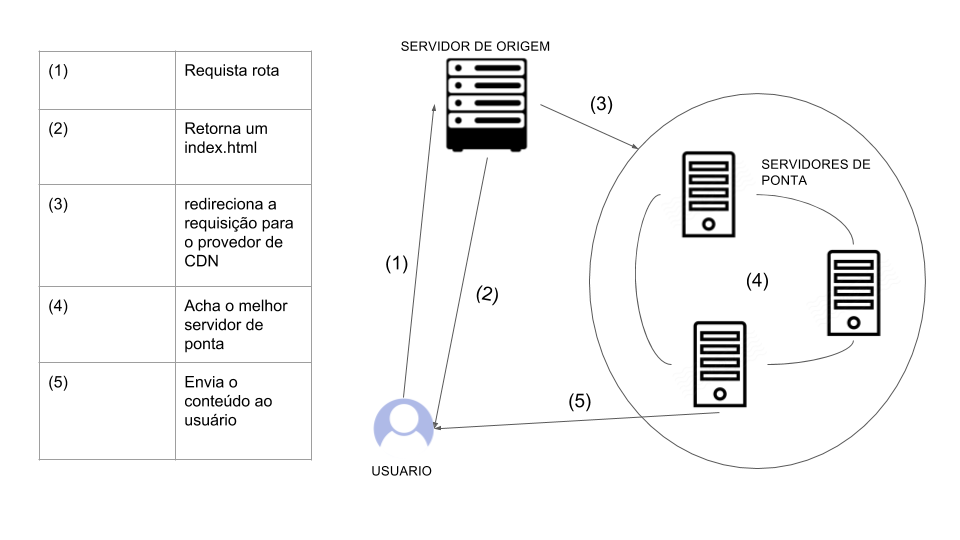
\includegraphics[width=13cm]{Figuras/entrega_conteudo.png} 
\label{figura:entrega_conteudo}
\end{figure}
\end{frame}
\subsubsection{Exemplo}
\begin{frame}{VOD - Video On Demand}{Envio da URL para o player}
\begin{figure} 
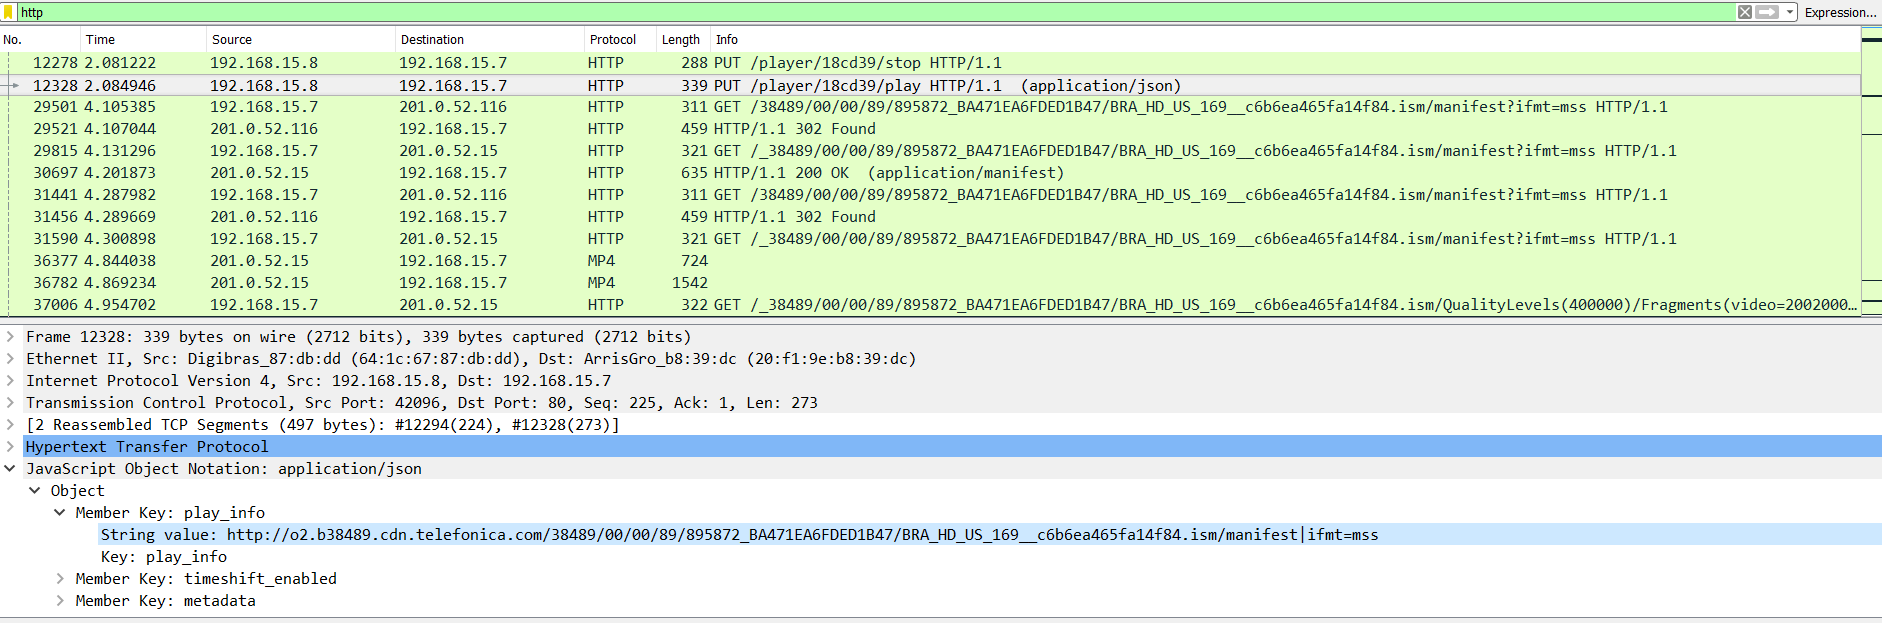
\includegraphics[width=13cm]{Figuras/exemplo_vod_1.png} 
\label{figura:exemplo_vod_1}
\end{figure}
\end{frame}
\begin{frame}{VOD - Video On Demand}{Get da URL para CDN}
\begin{figure} 
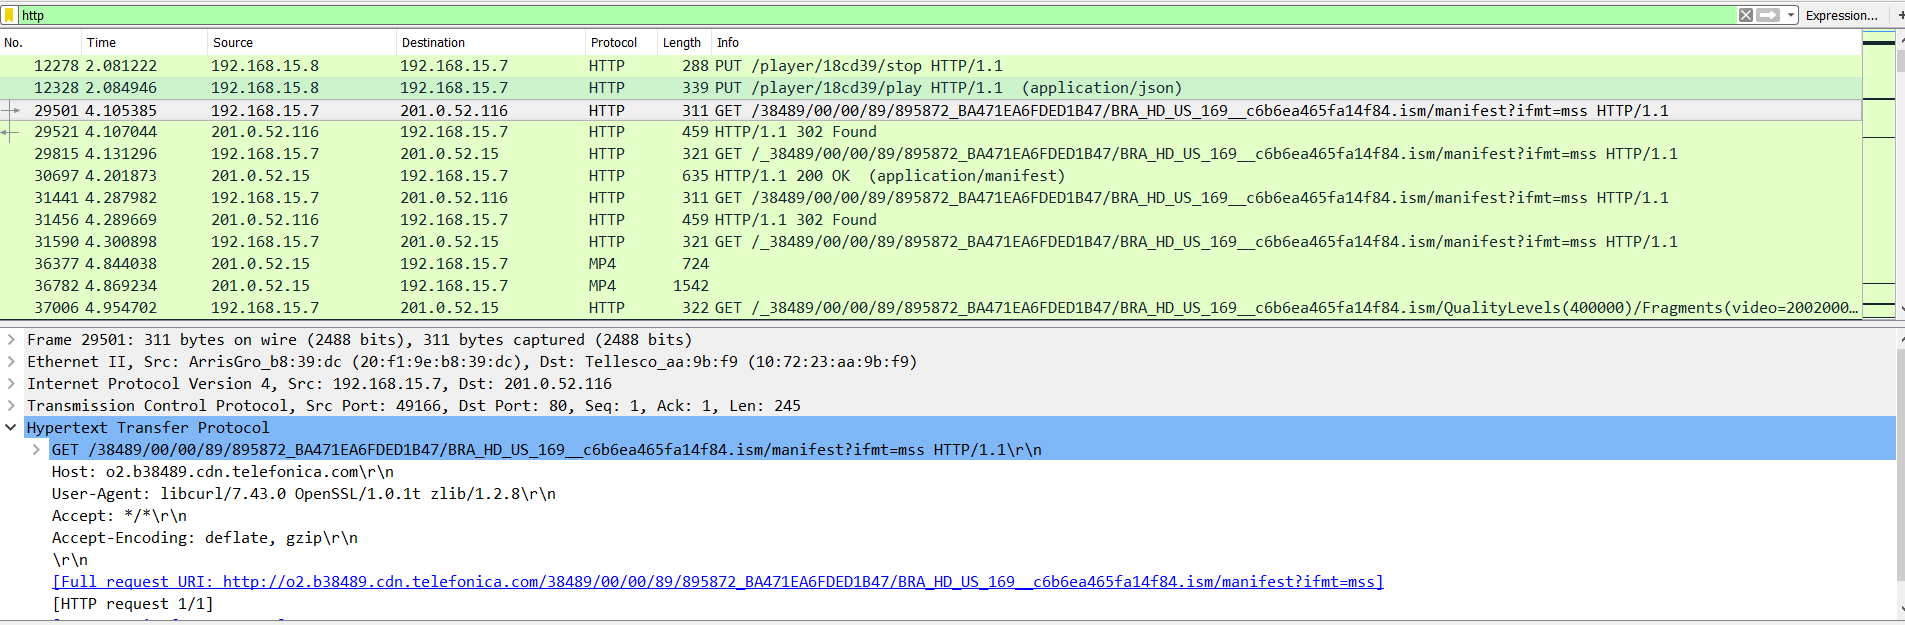
\includegraphics[width=13cm]{Figuras/exemplo_vod_2.png} 
\label{figura:exemplo_vod_2}
\end{figure}
\end{frame}
\begin{frame}{VOD - Video On Demand}{Retorno da URL no campo location}
\begin{figure} 
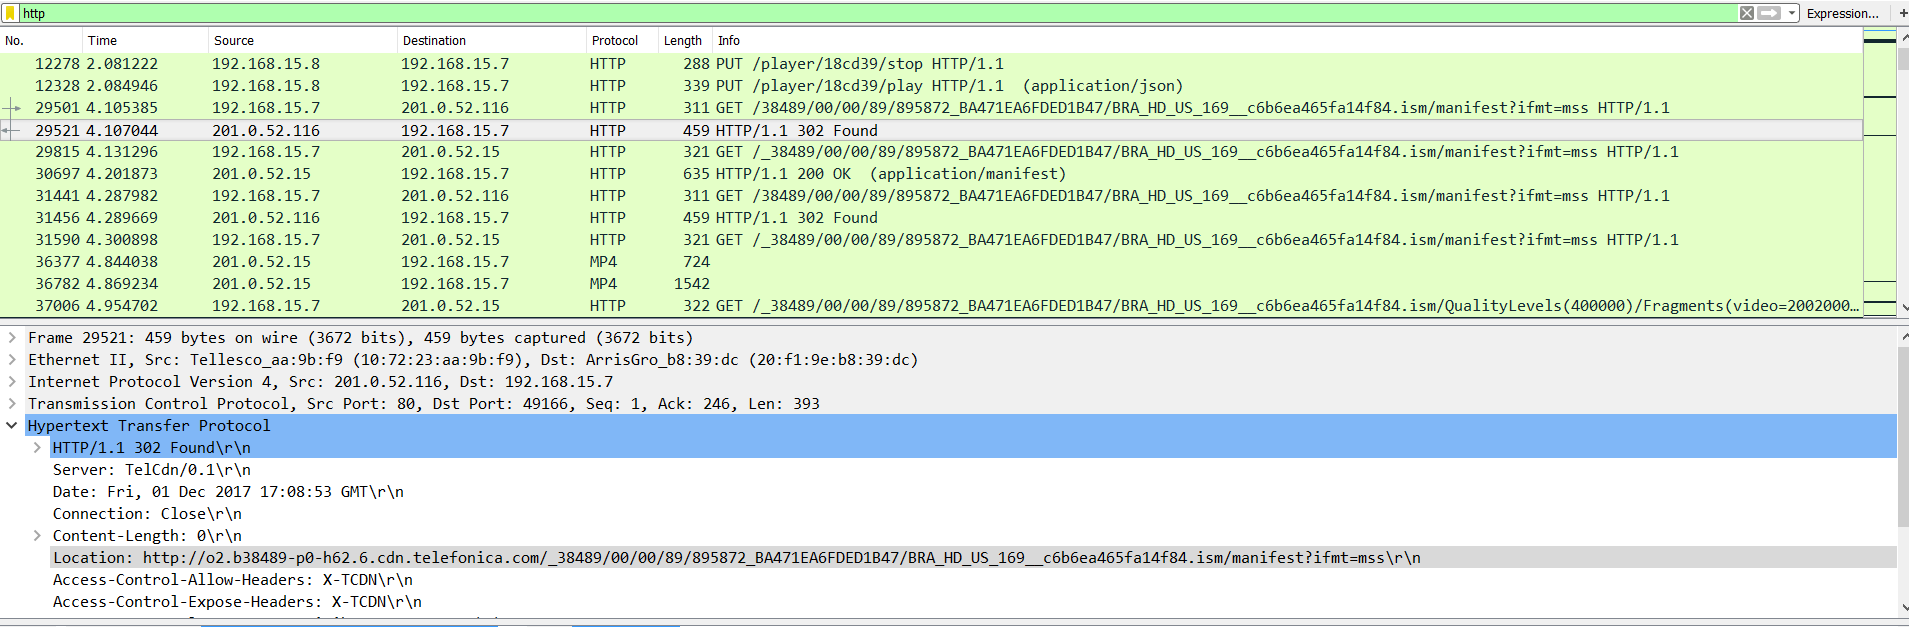
\includegraphics[width=13cm]{Figuras/exemplo_vod_3.png} 
\label{figura:exemplo_vod_3}
\end{figure}
\end{frame}
\begin{frame}{VOD - Video On Demand}{Download do chunck direto da URL}
\begin{figure} 
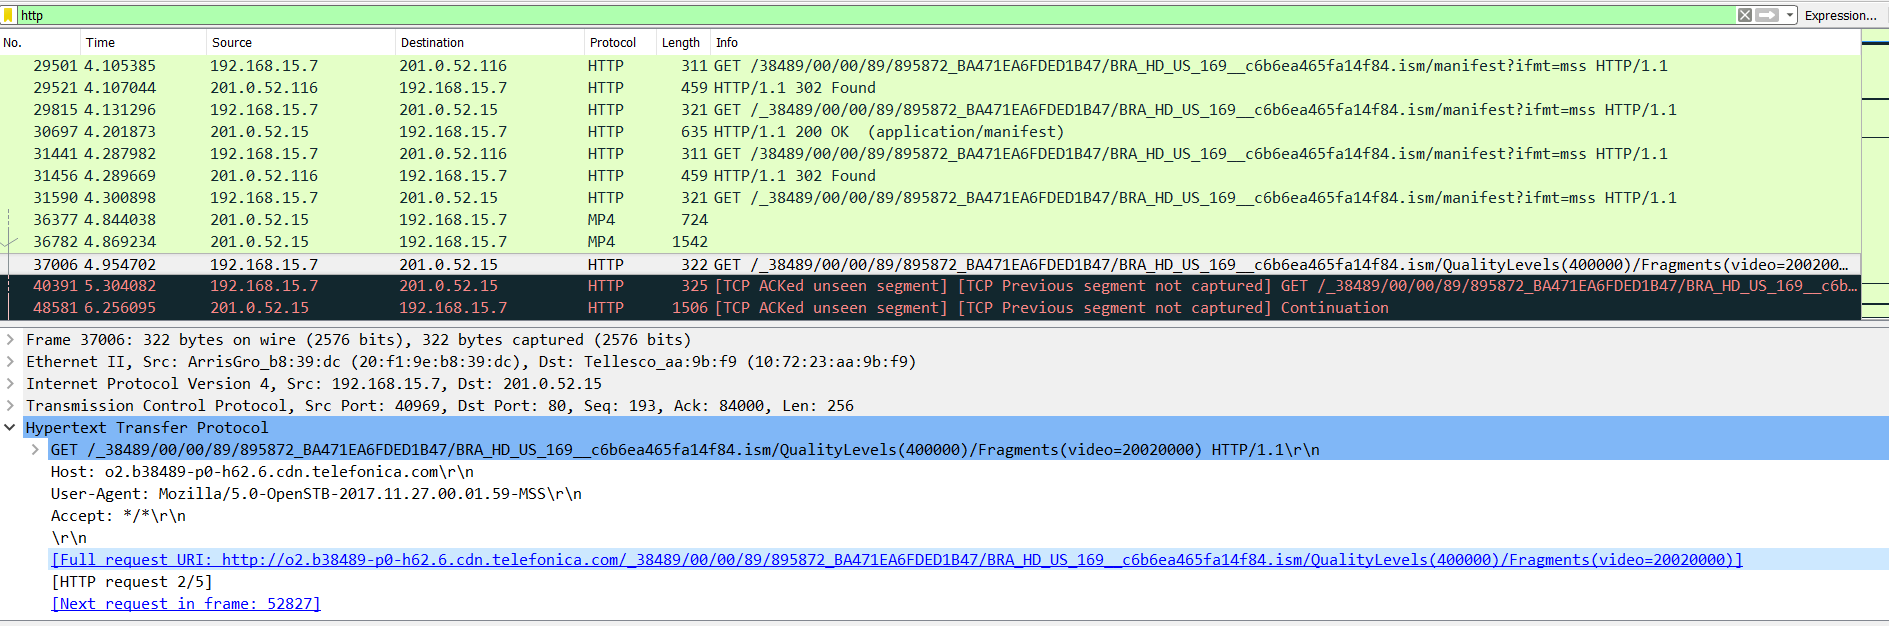
\includegraphics[width=13cm]{Figuras/exemplo_vod_4.png} 
\label{figura:exemplo_vod_4}
\end{figure}
\end{frame}
\subsection{Caching}

\begin{frame}{Caching}{Tipos}
\begin{itemize}
\item Intra-cluster
\begin{itemize}
\item Por pesquisa;
\item Por s\'intese;
\item Por diret\'orio;
\item Por hashing;
\item Por semi-hashing.
\end{itemize}
\item Inter-cluster
\begin{itemize}
\item Por pesquisa.
\end{itemize}
\end{itemize}
\end{frame}

\begin{frame}{Caching}{Intra-cluster}
\begin{itemize}
\item Por pesquisa:
\begin{itemize}
\item Uma pesquisa(consulta) \'e enviada de um cache para outro;
\item Lat\^encia \'e um problema;
\item Alto tr\'afego de informa\c{c}\~ao;
\item Espera receber "HIT" ou "MISS".
\end{itemize}
\item Por s\'intese:
\begin{itemize}
\item Cada servidor mant\'em um resumo dos conte\'udos dos outros;
\item Todos os caches subescritos s\~ao informados sobre mudan\c{c}as;
\item Alto tr\'afego em casos de muitas atualiza\c{c}\~oes;
\end{itemize}
\item Por diret\'orio:
\begin{itemize}
\item Vers\~ao centralizada do por s\'intese - Apenas um servidor mant\'em as informa\c{c}\~oes de todos.;
\item As consultas s\~ao feitas apenas no servidor central;
\item Exposto a estrangulamento de rede e a um ponto de falhas.
\end{itemize}
\end{itemize}
\end{frame}

\begin{frame}{Caching}{Intra-cluster}
\begin{itemize}
\item Por Hashing:
\begin{itemize}
\item Um servidor mant\'em uma fun\c{c}\~ao hashing com as informa\c{c}\~oes da URL do conte\'udo e endere\c{c}os de IPs dos servidores da CDN;
\item Todos os pedidos s\~ao redirecionados;
\item Possui baixa complexidade de implementa\c{c}\~ao;
\item Maior efici\^encia no compartilhamento de conte\'udo.
\end{itemize}
\item Por semi-Hashing:
\begin{itemize}
\item Um servidor possui parte do seu armazenamento para a mesma fun\c{c}\~ao hashing do por Hashing;
\item Outra parte para cache dos conte\'udos mais pedidos;
\item Cria 2 n\'iveis de caches;
\item Voltado para armazenamento de conte\'udo multimidia;
\item \'E o mais eficiente met\'odo de distribui\c{c}\~ao de conte\'udo.
\end{itemize}
\end{itemize}
\end{frame}
\section{Seguran\c{c}a}
\subsection{Criptografia}
\begin{frame}{Criptografia}{Tipos de chaves}
\begin{itemize}
\item Sim\'etricas
\item Assim\'etricas
\end{itemize}
\end{frame}
% Chaves simetricas
\begin{frame}{Chaves sim\'etricas}
\begin{figure} 
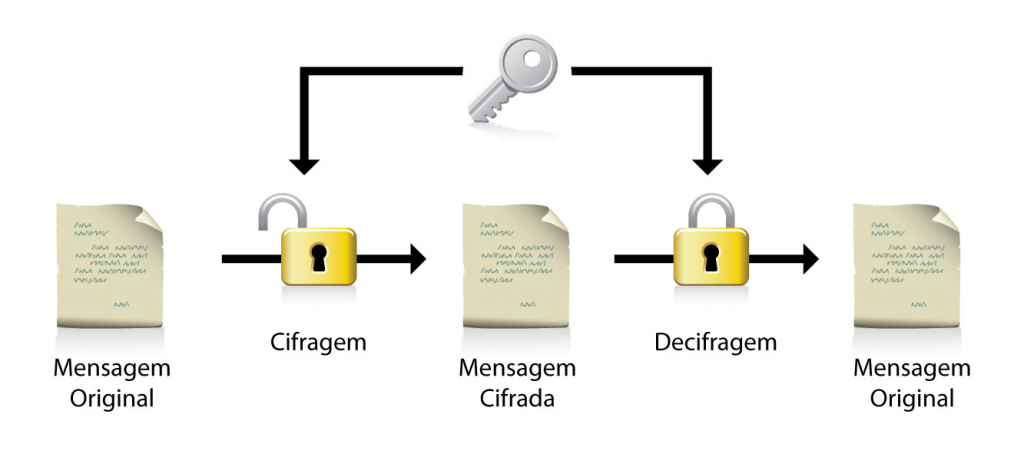
\includegraphics[width=10cm]{Figuras/criptografia_simetrica.png} 
\label{figura:criptografia_simetrica} 
\end{figure}
\end{frame}
\begin{frame}{Chaves sim\'etricas}{Algoritmos mais consider\'aveis}
\begin{itemize}
\item Cifradores de Vernam;
\item DES (Data Encryption Standard) -  Usa chave de 56 bits;
\item 3DES - Usa chave de 168 bits;
\item AES (Advanced Encryption Standard) - Usa chave de 128, 192 ou 256 bits;
\item A5/1, A5/2 e A5/3 - Criptografia de voz;
\end{itemize}
\end{frame}
% Chaves assimetricas
\begin{frame}{Chaves assim\'etricas}
\begin{block}{Acordo de chaves Diffie-Hellmann}
O acordo de chaves Diffie-Hellmann permite estabelecer uma chave secreta comum entre duas entidades, mesmo usando canais
de comunicação inseguros.
\end{block}
\end{frame}
\begin{frame}{Chaves assim\'etricas}
\begin{figure} 
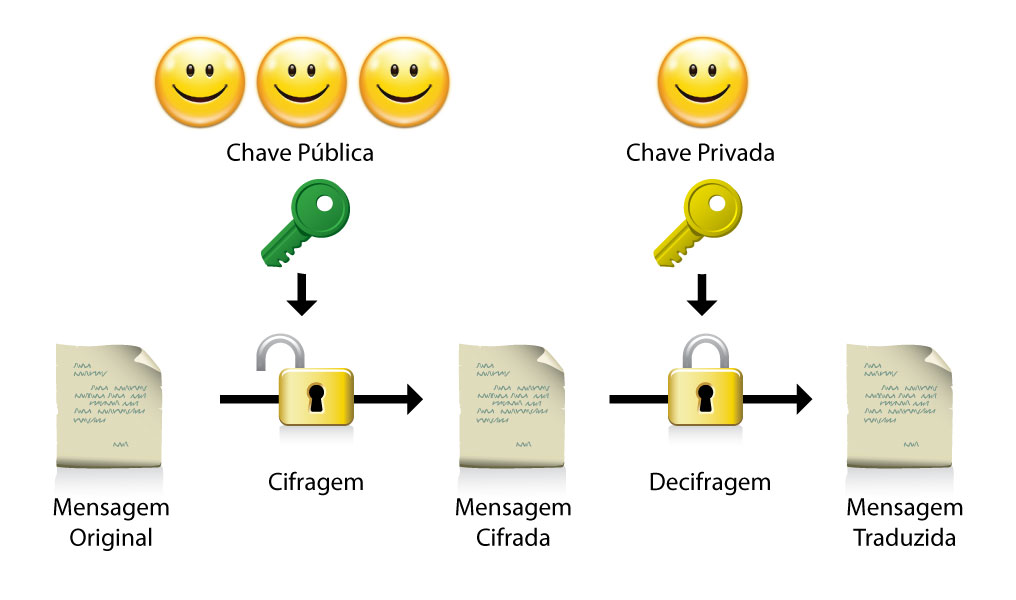
\includegraphics[width=10cm]{Figuras/criptografia_assimetrica.png} 
\label{figura:criptografia_assimetrica} 
\end{figure}
\end{frame}
\begin{frame}{Chaves assim\'etricas}{Aplica\c{c}\~oes}
\begin{itemize}
\item git;
\item ssh;
\item Assinatura digital;
\item Certificados digitais.
\item entre outros.
\end{itemize}
\end{frame}
\subsubsection{Exemplo}
\begin{frame}{VOD - Video On Demand}{Prote\c{c}\~ao de conte\'udo}
\end{frame}
\subsection{Autentica\c{c}\~ao de usu\'ario}
\begin{frame}{Autentica\c{c}\~ao de usu\'ario}
Em um sistema a autentica\c{c}\~ao de usu\'ario pode se dar de 3 formas:
\begin{itemize}
\item \textbf{SYK – Something You Know} - Algo que voc\^e SABE. Ou seja, um sistema de login/senha.
\item \textbf{SYH – Something You Have} - Algo que voc\^e TEM. Ou seja, um token, um smart card, um cart\~ao magn\'etico, um c\'odigo de barras, etc.
\item \textbf{SYA – Something You Are} - Algo que voc\^e \'E. Ou seja, caracter\'isticas intrinsecamente associada ao usu\'ario.
\end{itemize}
Em uma CDN, exceto no protocolo SOCKS, o fornecedor do conte\'udo pode escolher de qual forma vai proteger o seu conte\'udo. Podendo alternar entre essses m\'etodos ou at\'e mistur\'a-los.
\end{frame}
\subsubsection{Exemplo}
\begin{frame}{IPTV}{Autentica\c{c}\~ao de usu\'ario}
\begin{figure} 
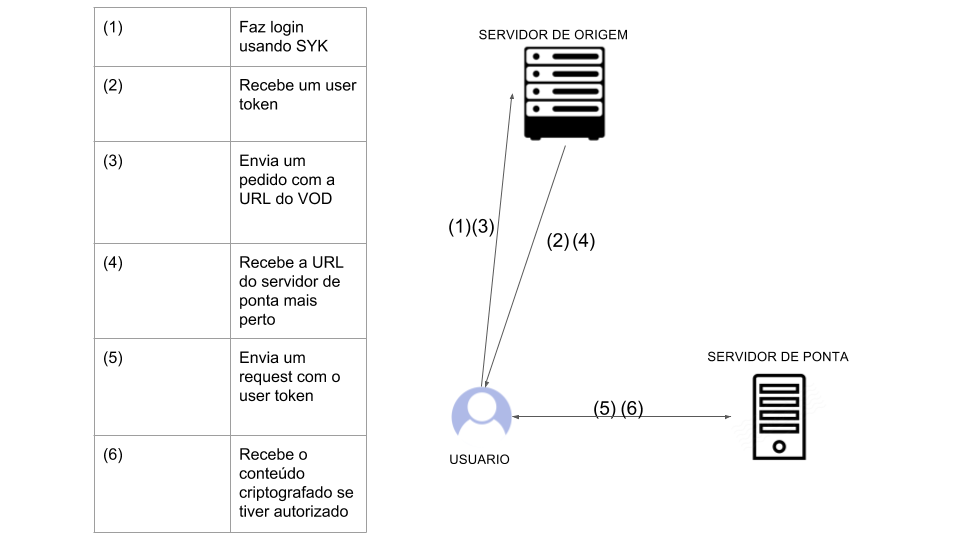
\includegraphics[width=13cm]{Figuras/autenticacao_vod.png} 
\label{figura:autenticacao_vod}
\end{figure}
\end{frame}
\section*{Anexos}

% All of the following is optional and typically not needed. 

\begin{frame}[t, allowframebreaks]
\frametitle{References}
\bibliographystyle{amsalpha}
\bibliography{references}
\end{frame}

\end{document}


